\documentclass[11pt,a4paper]{article}
\usepackage[hyperref]{emnlp-ijcnlp-2019}
\usepackage{times}
\usepackage{latexsym}

\usepackage{url}


  \usepackage{natbib}
  \bibliographystyle{plainnat}

\aclfinalcopy % Uncomment this line for the final submission

%\setlength\titlebox{5cm}
% You can expand the titlebox if you need extra space
% to show all the authors. Please do not make the titlebox
% smaller than 5cm (the original size); we will check this
% in the camera-ready version and ask you to change it back.

\newcommand\BibTeX{B{\sc ib}\TeX}
\newcommand\confname{EMNLP-IJCNLP 2019}
\newcommand\conforg{SIGDAT}

% Use the lineno option to display guide line numbers if required.

\usepackage{amsmath}
\usepackage{tikz-dependency}
\DeclareMathOperator*{\argmax}{arg\,max}
\DeclareMathOperator*{\argmin}{arg\,min}
\DeclareMathOperator{\E}{\mathop{\mathbb{E}}}

\usepackage{amssymb}% http://ctan.org/pkg/amssymb
\usepackage{pifont}% http://ctan.org/pkg/pifont
\newcommand{\cmark}{\ding{51}}%
\newcommand{\xmark}{\ding{55}}%

%\usepackage{pslatex}
%\usepackage{latexsym}
\usepackage[english]{babel}
\usepackage[utf8]{inputenc}
\usepackage{bm}
\usepackage{graphicx}
\usepackage{tikz}
\usepackage{xcolor}
\usepackage{url}
%\usepackage[colorinlistoftodos]{todonotes}
\usepackage{rotating}
\usepackage{multirow}





\usepackage[T1]{fontenc}

\usepackage{pslatex}
%\usepackage{latexsym}
\usepackage[english]{babel}
\usepackage[utf8]{inputenc}
\usepackage{amsmath}
\usepackage{bm}
\usepackage{graphicx}
\usepackage{tikz}
\usepackage{xcolor}
\usepackage{url}
%\usepackage[colorinlistoftodos]{todonotes}
\usepackage{rotating}
\usepackage{natbib}
\usepackage{amssymb}


\usepackage{amsthm}
 


\newcounter{theorem}
\newtheorem{proposition}[theorem]{Proposition}
\newtheorem{corollary}[theorem]{Corollary}
\newtheorem{question}[theorem]{Question}
\newtheorem{example}[theorem]{Example}
\newtheorem{defin}[theorem]{Definition}
\newtheorem{remark}[theorem]{Remark}
\newtheorem{lemma}[theorem]{Lemma}
\newtheorem{thm}[theorem]{Theorem}


\newcommand{\R}[0]{\mathbb{R}}
\newcommand{\Ff}[0]{\mathcal{F}}
\newcommand{\key}[1]{\textbf{#1}}


\newcommand{\soft}[1]{}
\newcommand{\nopreview}[1]{}
\newcommand\comment[1]{{\color{red}#1}}
\newcommand\mhahn[1]{{\color{red}(#1)}}
\newcommand{\rljf}[1]{{\color{blue}[rljf: #1]}}

\newcommand{\thetad}[0]{{\theta_d}}
\newcommand{\thetal}[0]{{\theta_{LM}}}
\newcommand{\thetap}[0]{{\theta_{P}}}


\title{On the Computational Capabilities of Self-Attention}
\author{Michael Hahn \\ Stanford University \\ mhahn2@stanford.edu}
\date{\today}
\begin{document}
\maketitle
\begin{abstract}
Transformers are emerging as the new workhorse of NLP, showing great success across tasks.
Unlike LSTMs, transformers process input sequences entirely through self-attention.
Previous work has suggested that the computational capabilities of self-attention to process hierarchical structures are restricted.
%Limitations of transformers are believed to exist; this work presents what appear to be the first formal proofs.
In this work, we mathematically investigate the computational power of self-attention to model formal languages.
Across both soft and hard attention, we show strong theoretical limitations of the computational abilities of self-attention.
Assuming natural input distributions, transformers cannot model periodic finite-state languages, nor basic recursion, with asymptotically better-than-chance cross entropy. % unless the number of layers or heads increases with input size.
%These results contrast with LSTMs, which can model many such languages perfectly.
We discuss implications of our theoretical results for natural language and NLP.
    %We show equivalences between transformers and classes of Boolean circuits, which entail strong limitations on the computational power of transformers.
    %First, we show that stacked argmax self-attention attention can only compute functions in $AC^0$, which entails strong limitations on the computations they can perform (compared to fully-connected networks).
    %Adding layer normalization, or using softmax self-attention, yields $TC^0$.
    %Complements recent work on the power of transformers.
\end{abstract}


Transformers are emerging as the new workhorse of NLP;
unlike recurrent models, they process long sequences in parallel, enabling considerably faster processing of very large inputs \cite{vaswani2017attention}.
Transformer-based models have achieved the state-of-the art in tasks such as language modeling, machine translation, and creating pretrained contextualized word embeddings.


%This poses the question of what kinds of structures they are capable of expressing, and what kinds of computations they are able to perform.
Transformers are based on self-attention, performing their computations in a largely parallel fashion.
This has allowed them to scale to very long sequences.
On the other hand, it has been suggested that this limits their expressiveness, as they cannot process input sequentially.
Experimental evidence suggests that transformers might not be as strong as LSTMs at modeling hierarchical structure.

In this work, we consider these questions from a theoretical perspective.
Formally, we consider the problem of language recognition, the task of classifying input strings as either belonging to or not belonging to a formal language.
We mathematically examine the classes of languages that transformers can recognize.
%: Transformer reads, and decides is the word in the language. Viewed as a seq2seq problem, with the target sequence being just TRUE or FALSE.

We focus on the ability of transformers to compute (1) regular languages, and (2) context-free languages containing hierarchical structure.
Our results entail show strong theoretical limitations of self-attention:
Transformers cannot model non-counter-free regular languages or languages containing unbounded recursion.


\section{Self-Attention}
Here we define self-attention following \cite{vaswani2017attention}.
We have an input $x_1,...,x_n$, where $x_i \in \mathbb{R}^k$ are input embeddings.
We furthermore have a sequence $p_1, p_2, ...$ of positional embeddings $p_i \in \mathbb{R}^k$. These can be computed through some predefined scheme, or could be learned for each position occurring in the training data.
Input and positional embeddings are combined (e.g., addition or concatenation) to vectors $y_i^0 = f(x_i, p_i)$.

A transformer has a fixed number $L$ of layers; the activations $y_i^k$ at position $i$ of the $k$-th layer ($k=1, ..., L$) are defined as follows.
Each layer has a set of $H$ attention heads; we first compute attention scores for the $h$-th head:
\begin{equation}
    a_{i,j}^{k,h} = f^{att}_{k,h}(y_i^{k-1}, y_j^{k-1})
\end{equation}
where $f^{att}_{k,h}$ is a function combining the activations from the previous level into an attention score.
In practice, this can be implemented e.g. using dot product or additive attention.
The final activation of the head is computed by weighting according to attention weights:
\begin{equation}
    b_{i,k,h} = \sum_{j=1}^n \hat{a}_{i,j}^{k,h} y_j^{k-1}
\end{equation}
where $$ \hat{a}_{i,\cdot} = \operatorname{softmax}(a_{i,\cdot}) $$
In the hard attention variant \cite{perez2019turing} , we take the actual maximum of attention values instead of softmax:
$\hat{a}_{i,j} = \delta_{j, \argmax_{j'} a_{i,j'}^{k,h}}$.\footnote{This requires an arbitrary setting when there are multiple positions with maximal attention weight; we will assume that the one occurring first in the sequence is chosen. Our analysis would also work under other schemes of resolving ties, such as random selection.}
The final activation at each position is then computed as
\begin{equation}
    y_i^k := f^{act}(y_i^{k-1}, b_{i,k,1}, ..., b_{i,k,H})
\end{equation}
where $f^{act}$ can be implemented as a fully-connected feedfoward network.

Following the construction of Seq2Seq transformer networks, in the decoder part we compute a softmax probability vector from the last activation $y_{n+1}^L$.

%We consider the problem of language recognition as in Weiss et al: a Seq2Seq model is tasked with transducing words in the language to $1$, and other words to $0$.
%To accomodate imprecision in computation, we will relax this to only demand that the result by separated from 0.5 by some constant $\delta$.


%Finite/infinite precision, hardmax/softmax




\section{Settings}

Theoretical investigation of the computational power of neural architectures can examine either the idealized case of infinite numerical precision, or the setting of finite precision.
RNNs, LSTMs
In practice, computers are finite and algorithms relying on unbounded precision might be infeasible to approximate with finite precision.
On the other hand, the theoretical idealization of infinite resources is often argued to be useful in the construction of mathematical theories.
For instance, asymptotic complexity theory relies on the limit of arbitrarily long inputs, and yet makes predictions that are largely highly relevant to practical computing.
Similarly, the finiteness of precision does not preclude recurrent neural networks  from behaving as if they could encode unbounded numerical information for all practical purposes~\cite{weiss2018practical}.
We focus on infinite precision transformers, showing that the capabilities of self-attention are limited even in the setting of infinite precision.
We discuss finite the precision setting in the Discussion, Section REF.
%Our theoretical results will confirm that the idealization of infinite precision can result in more realistic asymptotic characterizations of practically relevant behavior, and that the capabilities of self-attention are limited even in the setting of infinite precision.

Furthermore, there is a choice between modelling soft attention and hard attention \cite{shen2018reinforced}.
In practice, soft attention is much easier to train with gradient descent methods; however, attention typically concentrates on one or a few positions (CITE), and analysis of neural network attention focuses on the positions where attention concentrates, suggesting that attention behaves mostly like hard attention in practice.
The only prior study of transformers~\cite{perez2019turing} assumes hard attention.
We will therefore examine both of these settings.
%We will see that, if arbitrary activation functions are allowed, soft attention is significantly more powerful than hard attention.
%On the other hand, in the realistic setting where activation functions obey reasonable regularity conditions (satisfied by ReLU, Tanh, ...), hard and soft attention result in similar limitations.

\section{Related Work}

\paragraph{Prior Work on Transformers}
It has been a recurrent suggestion in the literature that transformers are restricted computationally, as they cannot process their input sequentially.
\cite{dehghani2018universal} suggested that transformers are restricted computationally, motivating their proposal of a variant with adaptive and unbounded number of layers.
They argued that transformers cannot compute functions that require sequential processing of input, without providing further details or proofs.
Our results provide an explicit formalization of these limitations.
Similarly, \cite{shen2018disan,chen2018best,hao2019modeling} have introduced extensions of transformers with recurrence.


Other studies have experimentally tested the abilities of transformers to learn structures.
Most related to our work, \cite{tran2018importance} compared the ability of transformers and LSTMs to learn hierarchical structure, specifically English subject-verb agreeement and evaluating logical formulas.
Based on their experimental results, they suggested that LSTMs are better at learning hierarchical structure.

\cite{yang2019assessing} experimentally investigated the power of self-attention to extract word order information, finding differences between recurrent and self-attention models; however, these were modulated by the training objective.

\cite{perez2019turing} theoretically studied the ability of Seq2Seq transformers to emulate the computation of Turing machines.
There is no contrast between their results and ours: While we consider transducing inputs to a single label (0, 1), they study the setting in which the transformer computes an unbounded number of autoregressive decoding steps, not bounded in the input length $n$.


\paragraph{Investigating the Power of Sequence Learning Architectures}
The computational power of recurrent neural networks has been a focus of study.
A particular focus has been on their ability to learn non-regular context-free languages, often thought to provide simple models of recursion and hierarchical structure as found in natural language.

A range of studies has experimentally examined the ability of recurrent networks to model counter languages such as $a^nb^n$ \cite{weiss2018practical,suzgun2019evaluating}.
Other work has experimentally studied the performance of reccurent architectures on learning to recognize well-bracketed strings, a similar but more challenging problem \cite{sennhauser2018evaluating,bernardy2018can}.

Recently, \cite{merrill2019sequential} theoretically studied several types of recurrent networks, showing that -- in the finite precision setting -- LSTMs recognize a subset of the counter languages, whereas GRUs and simple RNNs recognize regular languages.
%Inter alia, their results entail that LSTMs cannot model the multi-symbol Dyck language in the finite precision setting.


A related, though different, strand of research has investigated the power of neural networks to model Turing machines.
A classical result~\cite{siegelman1991neural} states that -- given unlimited computation time -- recurrent networks can emulate the computation of Turing machines.
Very recently, \cite{perez2019turing} have shown the same result for both (argmax-attention) Transformers and Neural GPUs.
The crucial difference between these studies and studies of language recognition is that, in \cite{siegelman1991neural,perez2019turing}, the networks are allowed to perform unbounded recurrent computations, arbitrarily longer than the input length.

Based on this insight, \cite{chen2017recurrent} have proven (un)decidability results for many properties of languages recognized by recurrent nets, partly on the basis of the classical result by \cite{siegelman1991neural}.

%Beyond sequence modeling, the expressivity of other types of neural architectures has also been studied extensively.



%\paragraph{Computational Complexity}
%Our work is also related to research in computational complexity, specifically the theory of Boolean circuits.
%Transformers are reminiscent of bounded-depth circuits -- these are circuits that computer in a finite number of layers of gates that stays bounded as the input size increases.
%A celebrated theorem \cite{furst1984parity} states that such circuits, using AND/OR and NOT gates, require a superpolynomial number of gates to compute \textsc{Parity}.
%An important difference to neural transformers is that such circuits compute over Boolean inputs, whereas transformers operate over vectors of real numbers, a potentially more powerful representation format.



\section{Two Formal Languages} % : \textsc{Parity}

We will analyze the ability of transformers to recognize formal languages, using two basic regular and context-free languages.
%\textsc{Parity}.


\paragraph{\textsc{Parity}} is the set of bit strings such that the number of $1$s is even.
This is a very simple regular language, recognized by a finite-state automaton with two states.
The regular languages form the lowest layer of the Chomsky hierarchy, and even simple RNNs can compute all regular languages.
All regular languages whose syntactic monoid contains a group are at least computationally as hard as \textsc{Parity}.
This means, if transformers cannot compute \textsc{Parity}, they cannot recognize regular languages except for the counter-free ones.

%This contrastsir ability to emulate finite automata is strongly restricted, compared even to simple RNNs.


%Why is \textsc{Parity} interesting?
%The reason is that, as we will show, Parity is a very simple instantiation of certain properties that make a large range of problems hard for parallel computation with a fixed number of layers.
%If transformers cannot compute \textsc{Parity}, it immediately follows that they also cannot compute various more complex functions:

A system that evaluates logical formulas (CITE) has to (among other things) be able to handle iterated negations.
Evaluating iterated negations is tantamount to counting whether the number of nested negations is even or odd.
If we know that transformers cannot compute parity, this entails that they also cannot evaluate logical formulas accurately.
\cite{tran2018importance} experimentally studied the ability of transformers to learn this language, finding that they did not perform as well as LSTMs.


%\textsc{Logical Formulas} is the set of Boolean formulas evaluating to True. Formally, we consider formulas using $\wedge, \vee, \neg$ and atomic \textsc{true}.
%\cite{tran2018importance} experimentally studied the ability of transformers to learn this language, finding that they did not perform as well as LSTMs.



\paragraph{\textsc{2Dyck}} is the language of correctly bracketed words consisting of `(', `[' and `)', `]'.
This language is a very simple model of hierarchical structure.
The Chomsky-Sch{\"u}tzenberger theorem states that any context-free language arises from a variant of \textsc{Dyck} with multiple types of parentheses through intersection with a regular language and homomorphisms.
Consequently, the ability of LSTMs to model \textsc{Dyck} has been an object of study \cite{sennhauser2018evaluating,bernardy2018can}.
As \textsc{1Dyck} is a deterministic counter language, finite-precision LSTMs are capable of perfectly modeling \textsc{1Dyck}; though they perform less well for versions with multiple types of parentheses \cite{sennhauser2018evaluating}, which are not counter languages any more.
In contrast, our theoretical results will show that transformers cannot model \textsc{Dyck} even with a single type of parentheses.



\paragraph{Probability Distributions}
Calculating cross-entropy requires defining distributions over input words.
For \textsc{Parity}, we simply consider the distribution over i.i.d. bitstrings of length $n$, and consider the task of predicting the label (odd or even) from the string.
For \textsc{LogicalFormulas}, we consider the uniform distribution over formulas of length $n$, again considering the task of redicting the label (TRUE or FALSE).
For \textsc{2Dyck}, we take a slightly different approach, taking the uniform distribution of well-bracketed prefixes of length $n$, and predicting the set of valid next characters, which is a subset of $\{(,),[, ]\}$.
We consider the problem of predicting the label from the input separately for each input length $n$, and consider cross-entropy as $n\rightarrow \infty$.


%Recognizing whether an expression is bracketed correctly is a basic example of a context-free language and of recursion. If transformers cannot compute parity, they also cannot decide whether long expressions are bracketed correctly.
%To prove this reduction, we first note that a transformer capable of deciding whether an expression is bracketed correctly can be converted into a transformer for deciding whether a string has more $1$s than $0$s. TODO actually not recognizing, but to say whether there can be a closing bracket

%Let a string be given, we then create versions $a'$ and $a''$ where $a'$ has zeroes replaced by some neutral letter, and $a''$ has its ones replaced by that.
%We then concatenate $a'a''$ and interpret zeroes as `(' and ones as `)'.
%This string can be completed to a correctly bracketed one if and only if there are at least as many `('s as there are `)'s.
%Second, we can reduce $Maj_x Maj_y (x\leq y)$ TODO unclear, might explode

%\paragraph{Finite-State Languages with Groups:} 




%\section{Finite Precision}
%We start by examining the case of finite precision.
%We interpret finite precision as meaning that only finitely many floting point numbers are distinguished.\footnote{An alternative interpretation is that numbers can be unboundedly large, but precision is limited, e.g., numbers are only distinguished in intervals of some $\epsilon$.}
%As \cite{perez2019turing} remarked, finite precision means that there are only finitely many distinct positional encodings, and the positions can be partitioned into a finite partition $\mathbb{N} = P_1 \cup ... \cup P_N$.

%In this case, an input word as processed by the network can be reduced to listing the numbers of 0's and 1's in positions belonging to each of the subsets $P_i$.

%Such a network cannot asymptotically model $a^nb^n$.

%Such a network also cannot model \textsc{Parity}, since the finite-precision activations ...

%show Parity is not in $Maj_2[un]$: this is actually relatively easy to show, we just have a finite number of bins, and have a numerically imprecise representation of how many are in each bin.

%This argument is quite 

%Finite precision may be an unrealistic assumption for asymptotic analysis:
%If positional embeddings have $d=100$ dimensions, they can robustly distinguish between $2^{100} \approx 10^{30}$ many positions, much more than the input length encountered in any practical NLP application.
%This motivates the study of infinite precision.





\section{Results for Hard Attention}

We will start our analysis of infinite precision with the study of hard attention~\cite{perez2019turing}.
We show that hard attention transformers cannot represent \textsc{Parity}, \textsc{Dyck}, or \textsc{BooleanFormula}.
To keep the results maximally general, our analysis will use combinatorial arguments and make no assumption about, e.g., activation functions and the norms of parameter matrices.
In fact, we do not even assume that the internal representations $y_j^k$ are vector-valued, as opposed to, say, discrete structures.

%\paragraph{General Formalization of Transformers}
%Each head depends on a finite number of activations in the previous layer (skip-connections) and the one argmax thing that was attended to.


%Our results will show that hard-attention transformers are not only unable to recognize these languages perfectly, they are also unable to 




\begin{figure*}[ht]
    \centering
    \begin{tabular}{llll}
    (a) & (b) & (c) & (d) \\
    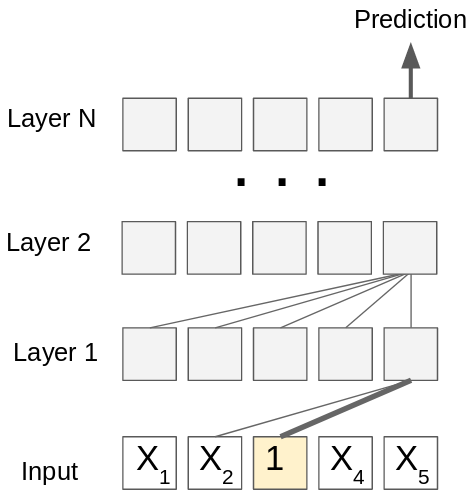
\includegraphics[width=0.23\textwidth]{figures/sa1.png} &
        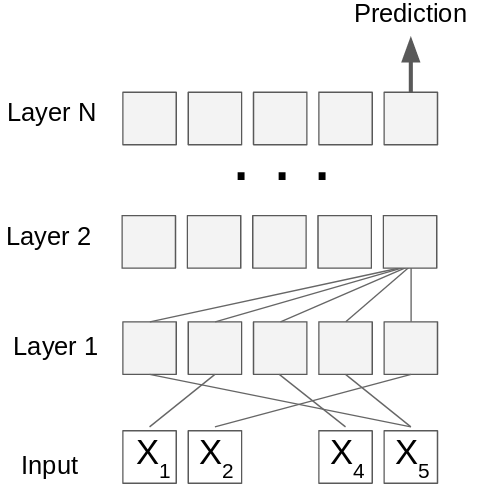
\includegraphics[width=0.23\textwidth]{figures/sa2.png}&
    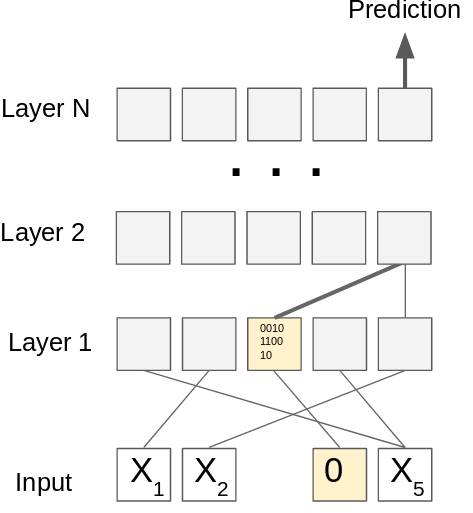
\includegraphics[width=0.23\textwidth]{figures/sa3.png} &
        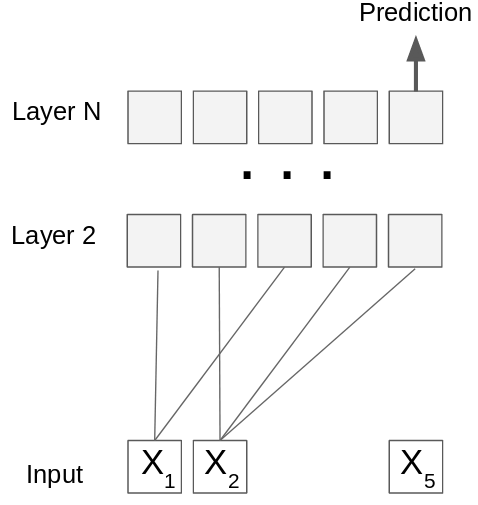
\includegraphics[width=0.23\textwidth]{figures/sa4.png}
        \end{tabular}
	\caption{Iteratively reducing the layers of a transformer by fixing a few input symbols. (a) We fix a small number of input symbols, `attracting' attention from the first layer to a few inputs. (b) After this step, each activation in the first layer only depends on a small number of input symbols. (c) We again fix a few input symbols in such a way as to `attract' attention of layer-2 heads to some layer-1 activations. As a result, each layer-2 activation only depends on a small number of layer-1 activations. (d) After this step, each layer-2 activation only depends on a few inputs, and we can remove layer 1. In this example, input $X_5$ ends up being ignored by the transformer after applying the restriction.}
	\label{fig:depth-reduction}
\end{figure*}


The basic idea (see Figure~\ref{fig:depth-reduction}) behind the proof is that, through fixing a small fraction of the input symbols in a particular way, we can `capture the attention' of the transformer in such a way that it ends up ignoring almost all remaining input symbols.
%More specifically, we will use the following approach.
%We take a transformer, and for each $n$, we consider what happens if we apply this transformer to inputs of that length.
%We show that, for large enough values of $n$, we can find a way to fix a small fraction of the inputs to 0 or 1, such that the prediction of the transformer depends only on a finitely bounded (independently of $n$) number of input positions.
%That is, after fixing these inputs, the transformer ignores a large number of inputs.
This shows that the transformer could not have solved a problem such as \textsc{Parity}, where every single input bit matters.
The idea of using such input restrictions is borrowed from the theory of Boolean circuits~\cite{furst1984parity,yao1986separating,hastad1994optimal}.
In particular, \cite{furst1984parity} used it to prove that polynomial-size bounded-depth Boolean circuits with $\wedge, \vee$, and $\neg$ gates cannot compute \textsc{Parity}.
We describe a new method to prove existence of suitable restrictions, as the proof approaches from the Boolean circuit literature do not seem to carry over to self-attention with infinite precision. %The proofs have in common the use of the probabilistic method, but the proof method in \cite{furst1984parity} does not appear to generalize to self-attention with infinite precision.


%Notably, our proof will not make any assumption about the nonlinearities, parameter matrices, positional embeddings, etc. -- all that is assumed is the basic self-attention architecture described above.
%We will not even assume that the same parameters are used for different input lengths $n$, only that the number of layers and heads is the same for all $n$.


%(On the other hand, for a problem such as AND or OR, fixing a single input is enough to fix the entire function, and transformers can do these easily indeed)
%\subsection{Preparation}
%We assume that there is only a single head per layer. If there are no restrictions on the number of layers, this is no loss of generality.
%We assume that, if two inputs have the same attention weight, the one with the smaller index is chosen. Our analysis would also work under other schemes of resolving ties, such as random selection.

An $n$-restriction $\rho$ is a map $\{1, ..., n\} \rightarrow \{*, 0, 1\}$.
After applying an $n$-restriction, the output value only depends on those inputs $x_i$ such that $\rho(i) = *$.

This will be the main technical result in this section, formalizing the intuition described above:
\begin{thm}\label{thm:hardmax-main}
Let any transformer be given, and let $C \in (0,1)$.
Then there is a family of input restrictions $\rho_n$ such that 
$$|\{i \leq n: \rho_n(i) = *\}| \geq Cn$$
%$\limsup_{n\rightarrow\infty} |\{i \leq n: \rho_n(i) = *\}| = +\infty$,
and such that the function computed by transformer on the restricted input depends only on a bounded number $c$ of inputs, independent of input length $n$.
\end{thm}
We first show how this entails that transformers do not recognize the three formal languages:
\begin{corollary}
Transformers with hard attention cannot model \textsc{Parity} or \textsc{Dyck}
with cross-entropy asymptotically better than chance.
%, or \textsc{BooleanFormula} (i.e., asymptotic cross-entropy is at chance level).
\end{corollary}
\begin{proof}
Take $C=0.1$.
For \textsc{Parity}, after applying a restriction, the output of the transformer depends on $c$ inputs.
An input of sufficiently large size $n$ thus has unrestricted inputs that do not influence the output.
But flipping a single input bit changes the value, so the transformer's output cannot match membership in \textsc{Parity} beyond chance as soon as $n$ is sufficiently large.

This directly entails that transformers also cannot do \textsc{BooleanFormula}.
TODO cross-entropy?

For \textsc{Dyck}, we first restrict the first $0.2n$ input positions to `('.
After applying the restriction provided by the theorem, the resulting restricted input will still be compatible with both well-bracketed and non-well-bracketed inputs.
As the prediction depends on only a bounded number of positions, this shows the transformer could not recognize \textsc{Dyck}.
TODO but cross-entropy?
\end{proof}

Our approach for proving Theorem~\ref{thm:hardmax-main} will be to iteratively remove the lowest layer of a given transformer by constructing input restrictions.
This process is illustrated in Figure~\ref{fig:depth-reduction}.
After the first step, each of the heads in the first layer will only depend on a bounded number $c$ of input positions.
In the second step, we apply the same argument to the heads in the second layer, so that each head in the second layer only depends on a bounded number $c'$ of heads in the first layer.
After this step, we can collapse the first layer into feedforward networks that transform a bounded number $\leq cc'$ of input positions into an activation $y_i^2$ of the second layer.
After this step, the first layer has been entirely removed.
Iterating this argument, we remove all layers.

After the removal of a layer, the resulting structure is not a transformer any more, as each head in the lowest layer now depends on a combination of input positions.
We introduce a technical definition to make this concept precise:

\begin{defin}[$c$-Augmented Transformer]
Let $c$ a positive integer. A $c$-augmented transformer of depth $d$ is one in which there is additionally a lower layer such that the laver-1 activations at each position are a function of only $c$ input positions.
\end{defin}

Note that an ordinary transformer  of depth $d$ is also a $1$-augmented transformer of depth $d$.

\begin{remark}
If we hit a transformer with $H$ heads with a family of restrictions that leave a linear fraction of inputs free, i.e.,
\begin{equation}
|\{i \leq n: \rho_n(i) = *\}| \geq Cn
\end{equation}
with $C \in (0,1)$, then we can also view the result as a transformer with $\operatorname{ceil}(1/C H)$ heads.

We can absorb the restrictions into the augmented transformers, and get (after renumbering the input size $n$, possibly throwing away duplicates for the same input size, and additionally restricting inputs to pad out gaps in the sequence) a sequence of $c$-augmented transformers, potentially with a larger number of heads.
\end{remark}
With this technical notion, we show that we can reduce layers, iteratively removing the lowest layer until no self-attention layer is left:
\begin{lemma}[Transformer Depth Reduction Lemma]
Given a $c$-augmented transformer. %with some restriction $\rho^0_n$ already applied, which hits a linear fraction of inputs (TODO clarify how this relates to having more heads).
We show that there is a family of input restrictions $\rho_n$ % extending $\rho^0_n$
such that
%$\limsup_{n\rightarrow\infty} |\{i \leq n: \rho_n(i) = *\}| = +\infty$
%(actually, it grows at most linearly)
\begin{equation}
|\{i \leq n: \rho_n(i) = *\}| \geq Cn %\frac{n}{10}
\end{equation}
for some $C \in (0,1)$,
and each second-layer head only depends on $ck$ inputs, for some constant $k$ independent of $n$.
\end{lemma}
Before proving this lemma, we note that it implies Theorem~\ref{thm:hardmax-main}.
\begin{proof}[Proof of Theorem~\ref{thm:hardmax-main}]
Apply the Depth Reduction Lemma iteratively, choosing the constants $C$ in the lemma small enough.
\end{proof}

%In particular, the resulting $c$-transformer can be rewritten into a $c'$-transformer with one layer removed.

%\begin{proof}
The rest of this section will be devoted to proving the Depth Reduction Lemma.
We will do the first part of the argument for any integer $k \in \mathbb{N}$.
In the second part, we will select a sufficiently large $k$.
%The aim is that $c' := ck$.

\paragraph{Preliminaries}
For the $i$-th level-1 head, we assemble for all inputs $j$ maximum attention value between head $i$ and input $j$ for the two possible inputs $0$, $1$.
Then we sort the inputs $j$ in descending order by maximum attention value: $j_1, j_2, ..., j_n$ (if there are ties, we order by position).
The following observation will be important: If we fix the input $j_k$ to the value that makes the attention value achieve the higher value, then the activation at element $i$ in level 1 only depends on the inputs $i, j_1, ..., j_{k-1}$.


For each layer-2 head, let $j_1, ..., j_n$ be the layer-1 elements downwards by the highest possible attention value that can be achieved for the given head.
We then select a subsequence $1 \leq i_1 < i_2 < ... < i_k \leq n$ such that (1) for each $i_s$, there is at least one input that only feeds into the element $j_{i_s}$ and no other $j_{i_s'}$, (2) $i_k$ is minimal, i.e. there is no subsequence with smaller $i_k$ that also satisfies (1).
There is only one case in which we cannot find such a subsequence, which is if all $j_1, ..., j_n$ together depend only on $< ck$ inputs, in which case this head already satisfies the condition we're aiming for.

A layer-2 head $k$-\textbf{depends} on some input $x_i$ if this input appears as an input to some $j_r$ for $r \leq i_k$.
A layer-2 head $k$-depends on an input if and only if that input appears as an input to some $j_{i_s}$ ($s \leq k$). (This is since $i_k$ is minimal).

Two layer-2 head are $k$-\textbf{neighbors} if some $j_{i_s}$ for one and $j_{i_s'}$ for the other both $k$-depend on some input $x_l$.

%We first show that, WLOG, we can assume that every layer-2 head has $\leq f = 2c^2k^2H$ many $k$-neighbors.
%We do this by creating a restriction that hits at most a linear fraction of inputs that enforces this.

%So let's assume there are heads with $f > 2c^2k^2H$ many neighbors (we do this argument for all values of $n$).
%Any head only depends on $\leq ck$ many inputs; by the Pigeonhole principle, this means,

We will construct input restrictions using probabilistic arguments over i.i.d. random restrictions.
For this approach to succeed, we require a  sufficient amount of independence between the activations of different heads in layer 2.
We thus need to ensure that the number of neighbors of each head is bounded.

Let $H$ be the number of attention heads in layer 2.
First, assume there is some input that has $>2kcH$ many $k$-depending layer-2 heads.
%We now show that the number of such inputs is small, and that we can remove those WLOG.
Assume the number of such inputs is larger than $0.9n$ for some $n$.
Then, the number of pairs of inputs and depending level-2 heads would be at least $0.9 n \cdot 2 H k c > Hckn$ for this $n$.
On the other hand, there are only $Hckn$ many pairs of inputs and depending level-2 heads -- contradiction.
Thus, the number of such inputs is at most $<0.9n$ for all $n$.
We can therefore construct restrictions $\rho_n$ that are set to some fixed value (doesn't matter which one) for these $<0.9n$ inputs, and to $*$ to others.
After this manipulation, every input has at most $2kcH$ many $k$-depending layer-2 heads, independent of $n$. %\footnote{For finitely many values of $n$ -- but by making $k$ larger after this manipulation, this will hold for all $n$.}


Furthermore, assume the number of inputs with $> 2cH$ depending layer-1 heads is $\geq 0.9n$.
Then the number of input to layer-1 connections is $>0.9n \cdot 2cH$.
But there are at most $ncH$ such pairs, contradiction.
So the number of inputs with $> 2cH$ depending layer-1 heads is $\leq Cn$ for $n$ large, for some costant $C \in (0,1)$.
We can restrict these inputs, again rewriting into a $c$-transformer with a potentially larger number of heads.


%Now consider those layer-2 heads that have $f > 2c^2k^2$ many $k$-neighbors.

%If there are $\leq n/(1.1c)$ many such heads (for some infinite subsequence of $n$'s -- we can throw away the other $n$'s -- for bad $n$'s, we just fix every input, and they'll drop out of the $\limsup$), then we can fix them manually, fixing only $\leq n/1.1$ many inputs. [I don't think we need this case -- the Case A below subsumes this, and doesn't presuppose the existence of many bad elements]

%So there are $> n/(1.1c)$ many such elements with $f > 2c^2k^2$ many neighbors (for all but finitely many $n$ -- we can throw away the other $n$'s).
%By the Pigeonhole principle, this means, there is some input that has $> 2kc$ many $k$-depending layer-2 heads.

%\begin{enumerate}
%\item Case A: the number of inputs with $\leq 2Hkc$ many $k$-depending layer-2-heads is $o(n)$ as $n\rightarrow\infty$, so the number of inputs with $> 2Hkc$ attached layer-2-heads dominates any linear fraction. Then, the number of pairs of inputs and depending level-2 heads would be at least $0.99 \cdot n 2 H k c > Hckn$ for $n$ sufficiently large. On the other hand, there are only $Hckn$ many pairs of inputs and depending level-2 heads.

%\item Case B: The number of inputs without $> 2kcH$ many $k$-depending layer-2-heads is $\Omega(n)$ as $n\rightarrow \infty$, in which case we can just fix these bad inputs (whose complement is asymptotically at least linearly large) to a fixed value. After this manipulation, $f \leq 2k^2c^2H$. We have hit only a linear fraction of inputs; by Remark above, we can rewrite this into a $c$-transformer with a potentially larger number of heads.
%\end{enumerate}

%NOTE:
%The number of pairs between input and level-2 heads is $\leq Hckn$.
%So the number of heads where that have more than $100 Hck$ attached layer-2 heads is $\leq n/100$.
%So we can make the fraction of replaced inputs very small.

%The number of heads that have to be satisfied is now $\leq Cn$, for some $C$ that was determined by the manipulations we made above. (this means that the restriction to one head per $n$ was unnecessary)

\paragraph{Constructing Restrictions}
After the previous part, we are in the setting where every input has $\leq 2kcH$ many depending layer-2 heads, and consequently every layer-2 head has at most $f \leq 2c^2k^2H$ $k$-neighbors (for any $k$).
(Note that the transformations carried out above could at most have increased the value of $H$).
Also, every input has $\leq 2cH$ depending layer-1 heads.

% after applying restrictions $\rho_n$ such that $\limsup_{n\rightarrow\infty} |\{i \leq n: \rho_n(i) = *\}| = +\infty$.
%Note that the previous part works for any $k$; we will choose a suitable $k$ in this section.

In order to prove the existence if suitable input restrictions, we apply the ``probabilistic method'': we define a probability distribution over restrictions $\rho'$ of inputs, and show that the probability mass assigned to restrictions of the type we require is strictly greater than zero, showing that such a restriction exists.

Define the distribution that independently assigns to each input the symbol $*$ with probability $p$, and $1$ or $0$ with equal probability else.
Define $X_i$ ($i=1, ..., H n$) to be the event that, for the $i$-th head, none of $j_1, ..., j_c$ are assigned the value that produces the higher attention weight (each of these is assigned either the other value, or $*$).
Define $X_0$ to be the event that more than $(1+\delta)qn$ many inputs are set to $0/1$.

We first show that the probability of $X_i$ decays exponentially in $k$.
Let $Y_i^t$ ($t=1,...,k$) be the event that the layer-1 head $j_{i_t}$ is not assigned the value that produces the highest attention weight.
Note that $X_i = \bigcap_t Y_i^t$.
We have $P(Y_i^s) = 1-(q/2)^c < 0$ (where $q = 1-p$).
Any $Y_i^s$ can be statistically dependent on at most $c \cdot 2cH = 2c^2H$ other events $Y_i^{s'}$.
Therefore, there is a set of $\geq \frac{k}{2c^2H}$ independent events among these.
Call these $Y_i^{t_1}, ..., Y_i^{\frac{k}{2c^2H}}$.
Then $X_i \subseteq \bigcap_{s=1}^{\frac{k}{2c^2H}} Y_i^{t_s}$, and thus
\begin{equation}
    P(X_i) \leq \prod_{s=1}^{\frac{k}{2c^2H}} Y_i^{t_s} = (1-(q/2)^c)^{\frac{k}{2c^2H}}
\end{equation}
%We use induction over $t \in \{1, ..., k\}$ to compute the probability that none of $j_{i_1}, ..., j_{i_t}$ are assigned to value achieving the maximal attention weight.
%At $t=1$, the failure probability for $j_{i_1}$ is $\leq (1-(q/2)^c)$.
%For $t+1$: Assume that $j_{i_{t+1}}$ introduces $w > 0$ new input variables not occurring in $j_{i_1}, ..., j_{i_1}$.
%Failure probability is $\leq F_t \cdot (1-(q/2)^w)$.
%TODO maybe this isn't actually strict enough
%\end{proof}
Furthermore, a Chernoff bound gives\footnote{See 
\url{https://en.wikipedia.org/wiki/Chernoff_bound#Multiplicative_form_(relative_error)}}
\begin{equation}
P(X_0) \leq    \exp\left(-\frac{\delta^2qn}{(2+\delta)}\right)
\end{equation}
We want to show that we can find $q \in (0,1)$, $A, B \in (0,1)$ such that the following holds, assuming $f \leq 2c^2k^2H$:
\begin{align}
 P(X_i) &\leq  C^k \leq A(1-B)(1-A)^f \\
P(X_0) &\leq \exp\left(-\frac{\delta^2qn}{(2+\delta)}\right)  \leq B (1-A)^{Hn}
\end{align}
Once we have this, then by the asymmetric Lov{\'a}sz Local Lemma \cite{mitzenmacherprobability}, there is some input restriction that avoids all events $X_0, X_1, ..., X_{Hn}$.

Choose $q=0.5$, $\delta=0.5$, $A=\frac{1}{2k^2c^2}$, $B=0.5$.
First, we need to satisfy
\begin{align}
    C &\leq A^{1/k}(1-B)^{1/k}(1-A)^{2kc^2} 
\end{align}
where $C$ is a constant in $(0,1)$.
For the RHS, 
$\lim_{k\rightarrow \infty} A^{1/k} = \lim_{k\rightarrow \infty} \frac{1}{k^\frac{1}{kc^2}} = \lim_{k\rightarrow \infty} \exp(-\frac{\log(k)}{kc^2}) = 1$.
Also, $\lim_{k\rightarrow \infty} (1-A)^{2kc^2} = \lim_{k\rightarrow \infty} (1-\frac{1}{CK^2})^{Ck} = \lim_{k\rightarrow \infty} (1-\frac{\sqrt{C}}{k^2})^{k} = 1$. So, if we choose $k$ large enough, the RHS can be made arbitrarily close to $1$, in particular, greater than the LHS.

In order to also satisfy
\begin{equation}
\exp\left(-\frac{\delta^2q}{(2+\delta)}\right)  \leq B^{1/n} (1-A)^H
\end{equation}
we calculate that the LHS is $<0.96$, and choose $n$, $k$ so large that $B^{1/n} > 0.99$ and $(1-A)^H = (1-\frac{1}{2k^2c^2})^H > 0.99$.

%Consider $A=2^{-a}$.
%So $2^{-a/k} (1-2^{-a})^{2kc^2} = 2^{-a/k} (\sum_{j=1}^a 2^{-j})^{2kc^2} = (\sum_{j=1}^a 2^{-j-a/{2k^2c^2}})^{2kc^2}$. After we have fixed $k$, we can adjust $a$ to make $a/{2k^2c^2}$ as small as desired to make the result be close to $1$.
%\end{proof}
This concludes the proof of the Depth Reduction Lemma.


%Can the same proof work for Dyck? Fix the first $0.2n$ to `(', and can we force the random restrictions to only restrict $0.3n$ (replace $2$ by $10$)?



\section{Results for Soft Attention}

%We first notice that, with arbitary activation functions, infinite precision softmax transformers:
%For simplicity, we consider languages over alphabets with only two elements, though the argument generalizes.
%Take positional embeddings $p_i = 2^{-i}$; and set $y_i^0$ to be $p_i$ if $x_i$ is $1$, and $0$ else.
%Then, by using an attention head that attends to each position with equal weight, we can compute $\frac{1}{n} \sum_{i : x_i = 1} 2^{-i}$.
%TODO

%In an actual transformer, all operations are Lipschitz.
%If we use additive attention, 
%If the norm of positional and input embeddings is bounded as $\|p_i\|_2, \|x_i\|_2 \leq p$, 
%The norm of activations in layer $k$ is bounded as $L^k p$.

In the previous section, we showed that transformers using hard attention are not able to recognize a range of core formal languages.

In this section, we study soft attention. %, where we will similarly show limitations of transformers in recognizing formal languages. %computing \textsc{Parity}, \textsc{Dyck}, and \textsc{LogicalFormulas}.
Here, we will use the smoothness of the operations used in transformers to show that any transformer, as inputs get longer, will not be able to robustly separate members of the languages from other inputs.
The idea behind the proof is that the impact of any single input on the output of the transformer is small if the input is long:
\begin{proposition}
If we exchange $l$ input bits, %a single input bit $x_i$ with the bit $x_i'$
then the change in the resulting activations at the decoder layers is bounded as $\mathcal{O}(\frac{l\cdot C^k}{n})$, where $n$ is the input length, $k$ is the number of layers, and $C$ is the norm of the parameter matrix.
\end{proposition}
This contrasts with recurrent networks:
Changing a single input can have nonnegligible impact on the final state even for very long input.
E.g., an RNN recognizing \textsc{Parity} through a hidden state that encodes parity of the current prefix will flip its hidden state if a single input bit is flipped.


This result entails that, as inputs become longer, soft attention transformers cannot achieve good cross-entropies, e.g., on \textsc{Parity} for i.i.d. coin flips:

\begin{thm}
Let a soft attention transformer be given for one of the languages \textsc{Parity}, \textsc{2Dyck}, \textsc{BooleanFormula}.
As $n\rightarrow\infty$, cross-entropy converges to chance level.
\end{thm}

\begin{proof}
TODO
\end{proof}

\begin{proof}[Proof of Proposition]
Let $D = \|x_i-x_i'\|_2$.
First, the difference in activations at this position is bounded as follows:
$\|y_i^0 - {y_i^0}'\| \leq L_f D$
where $L_f$ is the Lipschitz constant of the operation $f$ combining position and input embeddings.
Next, $\|y_i^1 - {y_i^1}'\| \leq L_{f^act} L_f D$

If $\|p_i\|, \|x_i\| \leq E$, then for activations $\|y_i^k\|_2 \leq 2 L_{f^act}^k L_f E =: F$.
Attention logits are bounded by $A := F^2 L_{f^{att}}$.
If attention logits are bounded as $|a_i| \leq A$,
then any attention weight $\exp(a_i)/\sum_j \exp(a_j)$ is upper bounded by $\frac{\exp(A)}{\exp(A) + (n-1) \exp(-A)} \leq \frac{\exp(2A)}{n}$.

Then, $\|y_j^k - {y_j^k}\| \leq C' k \frac{1}{n}$.

Thus the influence of any individual input on the final prediction is $\mathcal{O}(\frac{k}{n})$, with constants depending on the norms of parameter matrices.
\end{proof}


This shows that, as inputs get arbitrarily long, a soft attention transformer cannot robustly respond to small changes in the input.




This result stands in marked contrast to recurrent networks, where the impact of individual inputs on the final activation does not in general decay with sequence length.

In practice, we predict that soft attention transformers will need more layers and larger parameter values to solve formal languages like \textsc{Parity} on longer and longer inputs.





show the perplexity thing:

If the attention activations are bounded in norm by $L$ (which comes from the norms of the parameter matrices), then attention will ultimately be swamped, and asymptotically no individual element can have nonnegligible impact.

Here should have some experimental things


%\footnote{This result appears to contradict the claim in \cite{merrill2019sequential} that softmax asymptotically turns into the average of the attentions attended to most strongly. Our result shows that this would require }



\section{Discussion}

How do our results compare to what is known about LSTMs?
Recurrent networks such as SRNNs and LSTMs can perfectly emulate finite-state automata, and therefore can model finite state languages with optimal cross-entropy, as long as the state transition and symbol emission distributions are Markovian.
In particular, \textsc{Parity} of i.i.d. bitstrings can be predicted with zero cross-entropy, independent of the input length.
Infinite-precision LSTMs can model stacks \cite{kirov2012processing} and thus are theoretically capable of modeling \textsc{2Dyck} and \textsc{LogicalFormulas} perfectly.
On the other hand, the theoretical results of \cite{merrill2019sequential} show that finite-precision LSTMs cannot model these languages perfectly at long lengths.
Experimental evidence on the ability of LSTMs to learn \textsc{2Dyck} and \textsc{LogicalFormulas} from data is mixed, but clearly falls short of perfect accuracy or cross-entropy.




It is important to remark that all our impossibility results require taking large inputs:
Certainly, for any bound on the input length, we can construct a transformer that does anything we want.
However, we are interested in the extent to which a transformer is able to handle arbitrarily long inputs -- similar to analogous work on RNNs/LSTMs/GRUs.

Our results are consistent with the fact that transformer-based models tend to have far more parameters than comparable LSTMs (CITE).

While our hard attention results hold under extremely general assumptions, the analysis of soft attention builds on regularity properties of the operations that existing transformer models are composed of.
It would be interesting to investigate to what extent computational power increases when other operations -- e.g., discontinuous activations, or infinite attention logits -- are allowed.
One can show that the use of discontinuous activation functions such as the Heaviside function would enable perfect modeling of \textsc{Parity}; however, we do not know whether such changes would help with \textsc{2Dyck} and \textsc{LogicalFormulas}.\footnote{Analogy with Boolean circuits suggests that such results might be extremely hard to obtain: If transformers with soft attention were shown unable to compute \textsc{LogicalFormulas} even when allowing arbitrary activation functions, this would separate the functions computed by linear-size $TC^0$ circuits from the class $NC^1$, a widely believed but long open conjecture whose solution would be a major breakthough in computational complexity \cite{arora2009computational}.} % On the other hand, a proof that they can compute \textsc{LogicalFormulas} under such relaxations might translate into a proof that $TC^0$ and $NC^1$ coincide, }

...
We have shown that transformers cannot recognize regular languages that are not counter-free.
Since transformers have only linearly many activations in $n$, we conjecture that the class of regular languages recognized by transformers is $\bf{DA}$.


\paragraph{What does this mean for NLP?}


\section{Conclusion}


\bibliography{literature}


\end{document}

























\subsection{Step 1: Reducing first layer}
The first step will be to fix input values in such a value that each element in level 1 only depends on a bounded number of inputs, for some uniform bound $c$.

Take $c=20$.

Let $d$ be the maximum number of neighbors in level 1 (possibly $+\infty$).

If there are many neighbors, there is a straightforward way to construct a suitable input restrictions.
If the number of neighbors is small, we instead use probabilistic arguments to show existence of such a restriction.

\paragraph{Case 1} $d \leq 2c$.

We apply the ``probabilistic method'': we define a probability distribution over random restrictions of inputs, and show that the probability mass assigned to restrictions of the type we require is strictly greater than zero, showing that such a restriction exists.

Define the distribution that assigns to an input $*$ with probability $p$, and $1$ or $0$ with equal probability else.
Define $X_i$ ($i=1, ..., n$) to be the event that, for the $i$-th head, none of $j_1, ..., j_c$ are assigned the value that produces the higher attention weight (each of these is assigned either the other value, or $*$).
Define $X_0$ to be the event that more than $(1+\delta)pn$ many inputs are set to $0/1$.

We have\footnote{We get an inequality since it may happen that two input values produce the same attention weight}
\begin{equation}
    P(X_i) \leq (p + (1-p)/2)^c = (1/2 + p/2)^c
\end{equation}
and
\begin{equation}
P(X_0) \leq \exp(-\frac{\delta^2(1-p)n}{(2+\delta)})
\end{equation}
by a Chernoff bound.\footnote{See 
\url{https://en.wikipedia.org/wiki/Chernoff_bound#Multiplicative_form_(relative_error)}}


Take $A=0.01$, $B=0.5$, $p=0.5$, $\delta=0.9$.
Given also $c=20$, $n \geq 50$, the following bounds are true:

\begin{align}
\left(\frac{1+p}{2}\right) & \leq A^{1/c} (1-B)^{1/c} (1-A)^{2} \\
\exp(-\frac{\delta^2(1-p)}{(2+\delta)})  &\leq B^{1/n} (1-A)
\end{align}
Therefore ($d \leq 2c$),
\begin{equation}
\left(\frac{1+p}{2}\right)^c \leq A (1-B) (1-A)^d
\end{equation}
\begin{equation}
\exp(-\frac{\delta^2(1-p)n}{(2+\delta)})  \leq B (1-A)^n
\end{equation}


By the asymmetric Lov{\'a}sz Local Lemma \cite{mitzenmacherprobability}, there is some input restriction that avoids all events $X_0, X_1, ..., X_n$.

\paragraph{Case 2} $d > 2c$ 
WLOG this holds for infinitely many $n$'s (otherwise we can just remove them, and return to Case 1). in any case, we remove all non-initial $n$'s for which this doesn't hold.
Then we take one relevant chain, and reduce throughout.

(If the first unsatisfied $n$ doesn't have a participating head, then we can apply LLL there and be done with it)

In the next step, $d$ can at most have decreased.

\subsection{Step 2: Induction}

TODO this is copied from below


Let $c$ the number of inputs we got from Step 1.

Take $k$.
For each layer-2 element, we select a set of $\approx [k, ck]$ layer-1 inputs that in total use $k$ different input bits (If we can't, then this element is already $ck$-satisfied).

\paragraph{Case A:} There are boundedly many level-2 neighbors of these selected layer-2 elements ($f < 100 c k$ many).

Failure prob for a given layer-2 element is
\begin{equation}
\leq (1-q/2)^{k} (1-(q/2)^{c-1})
\end{equation}
\begin{proof}
TODO
\end{proof}
We want to obtain
\begin{equation}
    (1-q/2)^{k} (1-(q/2)^{c-1}) \leq A(1-B)(1-A)^f
\end{equation}
So we need
\begin{equation}
    (1-q/2) (1-(q/2)^{c-1})^{1/k} \leq A^{1/k}(1-B)^{1/k}(1-A)^{100c}
\end{equation}
We can make the LHS $(1-q/2) (1-(q/2)^{c-1})^{1/k} \approx 0.48$ with $q=0.99$ and $k=10$ (if $c=10$, greater $c$'s won't break it?! TODO).

Can we generally even get (works for $c=10, k=100$ at $c=10$, though it gets worse for $k = 10^{9}$)? Note that, for induction, we will need that $c$ can be unboundedly large. Can we just choose $A$ smaller and smaller for larger $k$?
\begin{equation}
    (1-q/2) (1-(q/2)^{c-1})^{1/k} \leq A^{1/k}(1-B)^{1/k}(1-A)^{2kc^2}
\end{equation}

Consider $A=2^{-a}$.
So $2^{-a/k} (1-2^{-a})^{2kc^2} = 2^{-a/k} (\sum_{j=1}^a 2^{-j})^{2kc^2} = (\sum_{j=1}^a 2^{-j-a/{2k^2c^2}})^{2kc^2}$. After we have fixed $k$, we can adjust $a$ to make $a/{2k^2c^2}$ as small as desired to make the result be close to $1$.

If $k$ is large enough in relation to $c$, then we can make the RHS large: First choose $A$ so that $(1-A)^c > 0.9$, then accept $k$ if $A^{1/k} > 0.9$ (else choose a larger $e$ to get a larger $k$).
And we can choose $B$ as small as we want (just make $n$ bigger in the second condition).

For the other element:
\begin{equation}
\exp\left(-\frac{\delta^2(1-p)}{(2+\delta)}\right)  \leq B^{1/n} (1-A)
\end{equation}

By making $A$ even bigger, we can make sure this is also true.

\paragraph{Case B:} There are $f > 100ck$ many neighbors for the inputs of the layer-1 set we selected, for infinitely many layer-2 sets.

(1) there is an unbounded number of elements (per $n$) that have less than $< 100ck$ neighbors -- we can apply LLL for this particular part of the input, and fill the other inputs arbitrarily. TODO but this might result in a too large number of filled inputs.

(2) there is only a bounded number of elements that have $< 100ck$ neighbors (for arbitrarily large values of $k$). 
Thus, asymptotically $>0.9n$ (say) of inputs are like this. But this can't be the case, as this would entail $90c  k n$ many under-consideration connections from input to second-layer when there are just $ckn$ many.

\subsection{Depth Reduction Lemma}

\begin{lemma}
Given: Transformer with first-layer fanin $c$. We show that there is a family of input restrictions $\rho_n$ such that $\limsup_{n\rightarrow\infty} |\{i \leq n: \rho_n(i) = *\}| = +\infty$, and each second-layer heads only depend on $c'$ inputs, for some constant $c'$ independent of $n$.
\end{lemma}

In particular, the resulting transformer can be rewritten into one with the second layer removed, and the new second layer having fanin $c'$.

\begin{proof}

Take $k$. $k$ will have to be chosen large enough for LLL to work. So we do the reduction to LLL for all $k$, and then choose $k$ large enough to make LLL work.

For each layer-2 element, we select a set of $\approx [k, ck]$ layer-1 inputs that in total use $k$ different input bits (If we can't, then this element is already $ck$-satisfied).

Now consider those layer-2 elements that have $f > 2c^2k^2$ many neighbors for the inputs of the layer-1 set we selected.

If there are $\leq n/(1.1c)$ many such elements, then we can fix them manually, fixing only $\leq n/1.1$ many inputs.


So there are $> n/(1.1c)$ many such elements with $f > 2ck^2$ many neighbors.
How do we get a contradiction?

- the number of inputs without $> 2kc$ attached layer-2-heads could be asymptotically infinite, in which case we can just fix these bad inputs (whose complement is asymptotically unboundedly large) to a fixed value, and then can apply LLL afterwards, as $f \leq 2k^2c^2$ then.

- the number of inputs without $> 2kc$ attached layer-2-heads could be asymptotically bounded, so almost all inputs have $> 2kc$ attached layer-2-heads. This is a contradiction, as this would entail $>ckn$ many such connections.

-------------------

After we previous part, we are in the setting where $f < 2c^2k^2$, and we apply LLL.



Failure prob for a given layer-2 element is
\begin{equation}
\leq (1-q/2)^{k} (1-(q/2)^{c-1})
\end{equation}
\begin{proof}
TODO
\end{proof}

We want to find that we can do find $q \in (0,1)$, $A, B \in (0,1)$ such that the following holds, assuming $f < 2c^2k^2$:
\begin{align}
    (1-q/2)^{k} (1-(q/2)^{c-1}) \leq A(1-B)(1-A)^f \\
\exp\left(-\frac{\delta^2(1-p)n}{(2+\delta)}\right)  \leq B (1-A)^n
\end{align}


\begin{proof}
We need to make

\begin{align}
    (1-q/2) (1-(q/2)^{c-1})^{1/k} &\leq A^{1/k}(1-B)^{1/k}(1-A)^{2kc^2} \\
\exp\left(-\frac{\delta^2(1-p)}{(2+\delta)}\right)  &\leq B^{1/n} (1-A)
\end{align}

Consider $A=2^{-a}$.
So $2^{-a/k} (1-2^{-a})^{2kc^2} = 2^{-a/k} (\sum_{j=1}^a 2^{-j})^{2kc^2} = (\sum_{j=1}^a 2^{-j-a/{2k^2c^2}})^{2kc^2}$. After we have fixed $k$, we can adjust $a$ to make $a/{2k^2c^2}$ as small as desired to make the result be close to $1$.
\end{proof}

-------

--------------
- there could be linearly many input elements with a large number of attached layer-2-heads, but we know the total number of such connections cannot exceed $ckn$ many.

- or there are only $o(n)$ input elements with so many attached layer-2-heads, in which 

%So there are $> n/(1.1c)$ many input elements with $> f/ck = 2k$ many attached layer-2 heads. So there are $2kn/(1.1c)$ many connections from input to layer 2, when there can be only $ckn$ many.




------------------------------------

The number of under-consideration pairs of connected input + second-layer head is $\leq ckn$.

So if there are $N$ many layer-2 heads with $Q$ neighbors, then there are $NQc$ many such pairs??? TODO this doesn't work

Asymptotically only $<\frac{0.5}{c} n$ of inputs can be like this: Assume otherwise, would entail $0.5/c \cdot c^2 k n = 0.5 c k n$ many  TODO fix this

Assume more than $0.1n$ of layer-2 head of $10000c^2k$ many neighbors.
For each such head, there is some input that is connected to $\frac{10000c^2k}{ck} = 10000c$ many layer-2 heads.
Also, there will be a linear number of such inputs, say $cn$ many such inputs each of which is connected to $100/c$ many layer-2 heads. (Note these constants all depend on how we chose $f$ to scale with $k$).

Can we just fix $k$ to be $10$ from the start, and take the factor $\frac{f}{k}$ to be some for which LLL still works? E.g., we know $\frac{f}{k} = 100c$ works, so that's actually $k^2 c$ if $k=10$.

So there are only $< 0.5/c  \cdot n$ many such bad layer-2 heads.
We can satisfy every one of these inputs, filling $\leq c \frac{0.5}{c} n \leq 0.5 n$ many inputs.

Once this is done, we only have layer-2 heads with less than $100ck = 1000c$ many neighbors, and we apply LLL.

Well actually, great values of $c$ don't seem to work for LLL. $k$ has to be chosen in dependence of $c$ (or $100c$, for that matter, so this won't work).

\end{proof}


%PROBLEM.
%maybe useful: $ k$ entails that there are exponentially more second-layer elements than input elements, which cannot be true for more than $\log n$ many input vars. so can we just fix $O(\log n)$ many such inputs and continue? Similarly for other sublinear functions in $k$. Can we show that for all but $o(n)$ many second-level elements, the number of relevant input elements grows somehow linearly in $k$, unless level 1 is somehow really degenerate???
%PROBLEM but if we replace $k$ by $\log k$ to make LLL work, this part here will break!?





\section{Step 1 (Reduce first layer)}

For each $c$ and each head, we take the $c$ distinct inputs that can achieve the maximal values for a certain input.

First start with small $c$, and go up until $c$ is large enough for LLL.

Case 1: Can apply LLL, $d \leq 2c$.

$\left(\frac{1+p}{2}\right)^c \leq A (1-B) (1-A)^d$

$ \exp(-\frac{\delta^2(1-p)n}{(2+\delta)})  \leq B (1-A)^n$



------------------

$\left(\frac{1+p}{2}\right)^c \leq A (1-B) (1-A)^{2c}$

$ \exp(-\frac{\delta^2(1-p)}{(2+\delta)})  \leq B^{1/n} (1-A)$


----------------------

$\left(\frac{1+p}{2}\right) \leq A^{1/c} (1-B)^{1/c} (1-A)^{2}$: e.g., for $c=20$, $A=0.01$, $B=0.5$, $p=0.5$

$ \exp(-\frac{\delta^2(1-p)}{(2+\delta)})  \leq B^{1/n} (1-A)$, e.g. for $\delta=0.9$, $n = 50$

-------------------------

Case 2: $d$ has gotten too large, say $d > 2c$.

WLOG this holds for infinitely many $n$'s (otherwise we can just remove them, and return to Case 1). in any case, we remove all non-initial $n$'s for which this doesn't hold.
Then we take one relevant chain, and reduce throughout.

(If the first unsatisfied $n$ doesn't have a participating head, then we can apply LLL there and be done with it)

In the next step, $d$ can at most have decreased.

--------------------------

Case 3: $d$ has gotten infinite: Deal with it as in Case 2.

------------------------------

Assume in the end there is only bounded number of free inputs (we never got into Case 3, and we never got into Case 1).
So we must get into Case 2 infinitely often, so for $n \rightarrow \infty$, the number of times we have applied Case 2 must have been infinite.



\section{Step 2 (Reduce second layer)}

Let $c$ the number of inputs we got from Step 1.

Let $e$ be the number of layer-1-inputs for each layer-2 element.

Claim: For each layer-2 element, we can find an independent set of some size $k$ unbounded growing with $e$ (in relation to $c$ which is bounded). [TODO prove -- not generally true: maybe all layer-1 elements refer to exactly the same inputs, or maybe they all share one input. \textbf{TODO have to get an estimate of failure probability that decreases exponentially in $k$ nonetheless, even if this happens.}]

(Exception: There may be units where we cannot get $k$ inputs, for the $k$ that we have chosen. Such units already satisfy the goal, their failure probability is just $0$)

Probability of failure: $(1-q^2/4)^k$.


As in Step 1, we increase $e$ until we succeed with one of the cases:


Case A: There are boundedly many neighbors ($f < c k$ many). (We only consider the neighbors of the independent set) (Even if they are not all independent, can take a maximal set of $k$ things where no two have exactly the same input, and failure prob is still something like $\leq (1-q/2)^{k} (1-(q/2)^{c-1})$, which should still be enough for LLL as $k \rightarrow \infty$. We can ignore cases of full overlap, as those won't count towards the number of relevant inputs) or do we better avoid the $\log k$ thing by constructing a maximal set of first-layer elements such that each one of them contributes some unique input element, as we want to just put everything into a bounded-width feedforward net, so all we need to bound is the number of input bits. (We can of course be in the special situation, where we cannot get $k$ to infinity, but then we can just fix the relevant inputs to remove these concerning elements (!?)).

PROBLEM the number of individual inputs (and thus independent observations) may just be $\propto \log k$! So we have $\leq (1-q/2)^{\log k} (1-(q/2)^{c-1})$. But then the number of neighbors also won't be a problem? So we have to somehow harmonize Case A and Case B to make sure this works.

\begin{equation}
    (1-q^2/4)^k \leq A(1-B)(1-A)^f
\end{equation}
So
\begin{equation}
    (1-q^2/4) \leq A^{1/k}(1-B)^{1/k}(1-A)^{c}
\end{equation}
We can make the LHS $(1-q^2/4) \approx 0.75$ with a very high $q$.

If $k$ is large enough in relation to $c$, then we can make the RHS large: First choose $A$ so that $(1-A)^c > 0.9$, then accept $k$ if $A^{1/k} > 0.9$ (else choose a larger $e$ to get a larger $k$).
And we can choose $B$ as small as we want (just make $n$ bigger in the second condition).

For the other element:

$ \exp(-\frac{\delta^2(1-p)}{(2+\delta)})  \leq B^{1/n} (1-A)$

By making $A$ even bigger, we can make sure this is also true.

Case B: There are $f > ck$ many neighbors for the inputs of the independent set.
TODO.

????

(1) there is an unbounded number of elements that have less than $< ck$ neighbors -- we can apply LLL for this particular part of the input, and fill the other inputs arbitrarily.

(2) there is only a bounded number of elements that have $< ck$ neighbors (for arbitrarily large values of $k$). 

WLOG there is an unbounded number of different inputs that all have $\geq 100c \log k$ (we can just take $100c  k$ throughout, instead of $c  k$) second-layer neighbors (else could just set them and forget about them). even, asymptotically $>0.9n$ (say) of inputs are like this. But this can't be the case, as this would entail $90c  k n$ many connections when there are just $ckn$ many?!
%PROBLEM.
%maybe useful: $ k$ entails that there are exponentially more second-layer elements than input elements, which cannot be true for more than $\log n$ many input vars. so can we just fix $O(\log n)$ many such inputs and continue? Similarly for other sublinear functions in $k$. Can we show that for all but $o(n)$ many second-level elements, the number of relevant input elements grows somehow linearly in $k$, unless level 1 is somehow really degenerate???
%PROBLEM but if we replace $k$ by $\log k$ to make LLL work, this part here will break!?

Case C: There are unboundedly many neighbors: Case B should be sufficient here.



\section{Discussion}

\paragraph{Comparison with RNNs, LSTMS, CNNs}

RNNs can do all regular languages.

Bounded-depth 1D CNNs cannot do all regular languages, they are even less powerful than transformers.

What are transformers better at than LSTMs?
Conjecture: where memory bottlenecks are relevant

\paragraph{What does this say about NLP and Language?}


\section{previous}



Let $e$ be the number of first-layer elements we want to consider for a given head.
That means, $ec$ input elements.

Let $f(e)$ be the number of neighboring second-layer heads. 

If $f(e)$ is infinite, or greater than $2ec$, it's not clear whether that's even useful?!

probability of bad event:
$1-((1-q)/2)^{c}$
obstacle here is that the first-layer elements are not independent, since they might use the same input bits.

can we do better on this?

%$q = 1-p$
%- no need to get all $c$ right, fixing the highest-ranking elements of these $c$ ones is enough: 1 (q/2), 01 (q/4), 001 (q/8), ....
%probability of getting the $c$'s right for a fixed one: $q \sum_{i=1}^c 2^{-i} = 1-\frac{1}{c}$
%probability of the bad event happening: $\leq 2^{-c}$

-------------------------

- if there is a large set of independent first-layer elements, then might still be good $(1-((1-q)/2)^{c})^{e}$ (this seems like a rare case, since $e$ would need to be large for this prob to be usefully small)

- can do induction? -- unclear


\section{draft}

Iterate:
Take the smallest $n$ which hasn't been solved.

Case A: there is a head for which $d$ really is so large, then process an entire chain through all $n$'s (just by setting $c$ variables, we can satisfy $1.5 c$ many heads. Satisfying all the remaining heads can only take fixating at most $n-1.5c$ variables).

Case B: there is no so head, can just apply LLL

Assume that the number of free things is bounded, then we did only go through A finitely often, but then we must have applied LLL, contradiction.


\section{previous ideas}

STEP 1: Reduce the first layer. Apply random restrictions + LLL.

$p$ is the probability that a variable is left unassigned.

Bad events:

(1) $A_i$: did not hit any of the top $c$ inputs with the relevant input

(2) $A_0$ have more than $(1+\delta)(1-p)n$ assigned variables

$P(A_i) = (p+(1-p)/2)^c = \left(\frac{1+p}{2}\right)^c$

$P(A_0) \leq \exp(-\frac{\delta^2(1-p)n}{(2+\delta)})$

$A$ assigned the $A_i$ events, $B$ assigned to $A_0$.


$P(A_i) \leq A B (1-A)^n$

$P(A_0) \leq B (1-A)^n$

so we have

$\left(\frac{1+p}{2}\right)^c \leq A B (1-A)^n$

$ \exp(-\frac{\delta^2(1-p)n}{(2+\delta)})  \leq B (1-A)^n$

Set $A_n := \frac{1}{2^n}$:


$\left(\frac{1+p}{2}\right)^c \leq \frac{1}{2^n} B (1-\frac{1}{2^n})^n$ (doesn't work!!!)

$ \exp(-\frac{\delta^2(1-p)}{(2+\delta)})  \leq B^{1/n} (1-\frac{1}{2^n})$ (this one's okay)


-------------------------------------------------


STEP 1: Reduce the first layer. Apply random restrictions + LLL.

$p$ is the probability that a variable is left unassigned.

Bad events:

(1) $A_i$: did not hit any of the top $c$ inputs with the relevant input

(2) $A_0$ have more than $(1+\delta)(1-p)n$ assigned variables

$P(A_i) = (p+(1-p)/2)^c = \left(\frac{1+p}{2}\right)^c$

$P(A_0) \leq \exp(-\frac{\delta^2(1-p)n}{(2+\delta)})$

$A$ assigned the $A_i$ events, $B$ assigned to $A_0$.

TODO wrong!?!? each can be dependent on more than $c$ different ones

$P(A_i) \leq A B (1-A)^c$

$P(A_0) \leq B (1-A)^n$

so we have

$\left(\frac{1+p}{2}\right)^c \leq A B (1-A)^c$

$ \exp(-\frac{\delta^2(1-p)n}{(2+\delta)})  \leq B (1-A)^n$

So 

$\left(\frac{1+p}{2}\right) \leq A^{1/c} B^{1/c} (1-A)$ (so choose $A$ close to $0$, and $c$ big)

$ \exp(-\frac{\delta^2(1-p)}{(2+\delta)})  \leq B^{1/n} (1-A)$ (so choose $A$ close to $0$)

Conclusion: The mass of good restrictions is at least

$\geq (1-B)(1-A)^n$

-------------------------------------------------

STEP 2: Reduce the second layer

For each element in the second layer, the probability that we hit at least one of the top-$d$ inputs is at least $((1-q)/2)^c$.
So the probability that we did not hit any of the inputs is at most $\leq 1-((1-q)/2)^c$.

$1-((1-q)/2)^c \leq AB(1-A)^d$ -- so we need $q$ to be really small

$ \exp(-\frac{\delta^2(1-q)}{(2+\delta)})  \leq B^{1/n} (1-A)$ -- again, need $q$ to be small

TODO feels wrong, too easy.

--------------------------------------------------

Probability that none is colored the right way, for one head: $(p+(1-p)/2)^d$.

We have $4d P(bad) \leq 1$ for small $d$ (unless $p$ gets bigger), so by Lovasz Local Lemma, there is a good assignment. TODO but how do we ensure that this doesn't just end up restricting everything?

(2) Now we just have to repeat this on the next level.

Probability that none is colored the right way: heuristically $(c(p+(1-p)/2))^d$. but actually things aren't independent. TODO problem


\section{Infinite Precision Transformers and Regular Languages}

Self-attention itself is compatible with recognition of any language in the sense of separating them!? just positional embeddings are $2^{-n}$, sum them up, and have very complicated nonlinear transformation of a few numbers in the output.
More interesting question is what can be implemented with e.g. a ReLU MLP.

\begin{proposition}
We can do parity with perfect accuracy, but not with perfect cross-entropy (neither with SoftMax not with ArgMax). At least if the nonlinearities are Lipschitz (does LayerNorm respect Lipschitzness?).
\end{proposition}
%take PARITY. want to get a final prediction. 

%take two inputs where the bags of input vectors are extremely close. or flip one input in an extremely long word.

(Problem: not clear how the proof would work with HardMax attention. But SoftMax has its own problem with long words. One way to deal with this is to modify Softmax by introducing a threshold below which a logit becomes minus infinity. But then cannot enforce that there will be nonzero values)

\begin{proof}
%Take an extremely long word, of length $n$, with $\approx n/2$ ones and zeroes.

Take some very long $n_\epsilon$.

Take three positions $i, j, k \leq n$ such that their embeddings differ only by $\leq \epsilon$.

Now consider the word where there are zeros everywhere, except for $i$, or except for $i$ and $j$.

The first level will also only differ by $\leq C \epsilon$.

Now take attention weight of $i,j,k$ with some other $l$. They can differ only by $\leq C' \epsilon$.

Take softmax over attention weights, again attention weights differ only by $\leq C'' \epsilon$.

Also the summed up things will be almost the same. And so on.

TODO LayerNorm. (the SDs will also be almost the same)
\end{proof}

Contrast this with RNNs: they can do any regular language easily

In fact, transformers can't even do AND/OR well, since many small attention weights will ultimately drown out one big one. Cam change this to HardMax attention.

QUESTION: Regular languages computable by HardMaxAtttention: $FO_2[<]$ ? HardMaxAttention can do all languages in this. Can it do additional ones?

Equations of $DA$: $(xyz)^\omega y (xyz)^\omega = (xyz)^\omega$

Also DA: $Me^\omega M \subseteq MsM$ imply $e^\omega s e^\omega = e^\omega$



How about $(ab)^*$? cannot do this either (this is not in $FO_2[<]$)

\section{Experiment: Transformers and Parity, requires large weights}

\section{Finite Precision, Argmax}

Finite precision transformers are related to Boolean circuits with bounded depth, linear number of gates, and very strong uniformity.

\begin{proposition}
Can at most do languages of this and that type (not restricted to regular, but extremely restricted).
\end{proposition}

- finite precision and argmax: AC0 with unary predicates and linear gates

\section{Finite Pecision, Softmax}

- finite precision and softmax: Majority with two variables and unary predicates

actually extremely restricted

\section{infinite precision and argmax}: ? TODO?

- infinite precision and softmax (can use a rational approximation to softmax!?) (certainly cannot do good in the sense of cross-entropy, though perhaps hard to prove for arbitrary positional encodings. accuracy more challenging)

-- what can we say about the predicate class?

-- something about cross-entropy:

conjecture Furst-Saxe-Sipser like result


----------------------

result

- transformers can do some basic recursion: $a^nb^n$ with neutral letter, single-Dyck (can use attention map to illustrate how it's done)

they can in the sense of argmax-accuracy

but can they also do it with optimal cross-entropy? (modulo a bound on the weights) (e.g., in the sense of perfectly saying whether the word is valid or not, for some length distribution with infintie support)
a thresholding thing cannot really do this. so less powerful than an LSTM!?

- formally, transformers sorta coincide wtih $LTC^0$

-- presumably cannot do multi-Dyck!? (or even multi $a^nb^n$ with neutral letter) (can argue that LSTMs cannot do this either)

(BUT if the goal is just to say, assuming wellformedness, predict the one next thing, then it works. this is different from recognizing though, which would rquire quadratically many hedas.)

- neither can do logical formulas (assuming widely believed circuit lower bounds)

- on the other hand, there are regular languages that transformers cannot do (assuming those lower bounds)

- we also show that transformer's ability to do any kind of recursion crucialy relies on the use of soft -- as opposed to hard -- attention.
indeed, without soft attention, can do neither $a^nb^n$ not parity

- is there something where transformers are better than LSTMs?

(-- boring: things that can be solved by looking at positions, such as $a^nb^n$)

-- without counting or infinite precision, LSTM memory scales with number of units. for transformers, bottleneck is instead the ease of retrieving and combining info.

-- example? high crypticity process where everything MIGHT become relevant, but one doesn't know whether it will. e.g., $X_t$ informs which aspect of the past is relevant for $X_{t+1}$. as long as one can then also retrieve this part from the past, this is useful. maybe can do some actual language modeling thing where this matters. e.g. carrying around a lot of names.



transformer cannot do anbn version with two letters
\begin{proof}
we formalize transformer with order + unary
\end{proof}


on the other hand, actually LSTMs can use fractal encoding of stack

transformer cannot do such a thing. specifically, cannot do two-bracket neutral letter anbn. for simplicity can do incremental prediction. can you flesh out this argument?



LSTMs cannot do the anbn version with two letters
\begin{proof}
We work in the finite precision setting assumed by Weiss Goldberg ... 2018.

Note that at finite precision $h_t$ assumes finitely many values.

$c_t$ is a number (integer + remainder from a finite set). At each step, multiplied by $f_t$, and a finite value in $[-1,+1]$ is added.
If this multiplier $f_t$ is not saturated unboundedly often for some dimension of $c$, then this would destroy information.
Consequence: LSTM can only really do finite state + counting + multiplication with one of these numbers.

also control is saturated if c is really large, so always have to have some small c that reflects what to do next. but 
\end{proof}


issue: fixed transformer cannot simulate hard max over unboundedly long sequences, need to get larger and larger parameters to still enforce.

transformer cannot do anbn+neutral with perfect perplexity
\begin{proof}
at least heuristically, a single thing can't contribute much
\end{proof}



-----------------------------------

The success of transformers poses the question of what kinds of things they're capable of representing.
There is quite a range of studies on LSTMs/GRUs/SRNNs from this perspective, but nothing on transformers.
We examine the power of self-attention from a formal languages point of view, and compare to LSTMs.

(1) transformers can do basic recursion, and this ability crucially relies on the presence of soft (as opposed to hard) attention. in fact, with hard attention, they couldn't even count modulo 2. also, their ability to do this is a bit restricted compared to LSTMs (perplexity has to worsen with length)

(2) as it gets more complicated, neither transformers nor LSTMs work -- at least in the finite precision setting (Weiss et al. setting).
In particular, neither can do logical formulas (generally, neither of them can do a stack).
We show this by a combination of experiment, proof for LSTM, reduction to widely believed conjecture for transformer.

(3) there are regular languages that transformers cannot do (assuming this conjecture).

(4) we exhibit languages/processes that transformers do better on than LSTMs.



------------

- transformers have been tremendously successful in NLP

-- bert, gpt

- question what they (can) learn 

-- what are their limits?

-- how much of linguistic structure as linguists have identified can they encode?

-- how can we improve NLP?

- for more `traditional' recurrent models, some understanding

- some work on understanding transformers

- big problem for experimental work: hyperparameters

- we address this question:

- drawing on computational complexity

- will show limitations of transformers

-- with hard (argmax) attention, they are extremely limited: cannot do modulo counting, cannot do recursion

-- with softmax, they are more powerful, but -- if widely believed conjectures in computational complexity are true -- still cannot do more complex recursive tasks such as evaluate logical formulas

- show equivalence between transformers and certain classes of boolean circuits

- as a consequence, we transfer a host of results from computational complexity to transformers

- intuitively, transformers should not be able to do counting etc. We confirm this mathematically.

- experimentally

-- parity

-- recursion $a^nb^n$ with neutral letter

- We argue that our results have implications both for NLP and for linguistics.

- For NLP, our result confirms the idea that transformers cannot do recursion

- For linguistics, our results highlight an interesting question:
transformer-based models are the best quantitative models we have of language, but they are formally incapable of representing unbounded recursion -- reputedly a core property of language

Note that this is even stronger than with LSTMs:
LSTMs can do $a^nb^n$, transformers cannot (if there is a neutral letter).

- what to make of this?

-- language has recursion, but high depth is relatively infrequent, maybe due to human memory limitations



---------

It has been suggested that self-attention is computationally restricted, and (REF) proposed the universal transformer to address limitations.

No formal proof of the limitations, even though it seems intuitively plausible.

We show:
- Stacked self-Attention is strongly limited, coinciding with $FO[unary]$.

- Layer normalization and softmax self-attention both yield class coinciding with $TC^0[unary]$.
Widely believed to not be able to compute recursive things (such as evaluating logical formulas), BUT proving limitations on such architectures would be a breakthrough, so unlikelu.


\section{Introduce Transformers in more detail}

\section{Bounded-Depth Circuits}

FIGURE

In full generality, a Boolean circuit is a directed acyclic graph in which each vertex is labeled with some Boolean operation, and where the input and output vertices each are numbered.

Here we will mainly be concerned with circuits having $\wedge, \vee, \neg$, but one can construct circuits using other Boolean operations.

Clearly, circuits have a lot in common with feedforward networks, and the relation to quantized neural networks is particularly clear.
Also, a finite-precision feedforward net is a circuit.

Note a circuit -- like a feedforward net -- has fixed-dimensional input.

A circuit family assigns a circuit with $n$ inputs to each $n \in \mathbb{N}$.

A language is a set $L \subset \{0,1\}^\omega$.
A language is recognized by a circuit family iff ...

$AC^0$ is the class of languages recognized by circuit families that have (1) bounded depth, (2) polynomial size.





Parallel computation has been studied a lot

Circuit complexity

Some strong lower bounds.
In particular, FSS theorem. also some more things.
Before we show that these results

Our main technical result will be a reduction between (bounded precision) transformers and such $AC^0$ circuits.


Before we prove this, we discuss what this will give us.

Research has already identified lots of properties about the power of $AC^0$.

$AC^0$ circuits can deal with some simple properties

-- is there a 1 before a 0?

-- ...



The celebrated Furst-Saxe-Sipser theorem states that $AC^0$ circuits cannot recognize the \textsc{Parity} language, the language of bitstrings of even parity:
$$Parity = \{w \in \{0,1\}^n : n \in \mathbb{N}, parity(w) = 0\}$$
That is, in order to recognize this language, circuits using only and/or gates have to either grow in depth or become exponentially wide as $n$ increases.

As an example for the relevance of \textsc{Parity} for natural language:
Being able to solve \textsc{Parity} is a first prerequisite to evaluating logical formulas (due to iterated negation), and it is thus unsurprising that $AC^0$ cannot evaluate logical formulas.

In fact, $AC^0$ circuits cannot do recursion at all, beyond a trivial level:
They can do $a^nb^n$, but they cannot do the version of $a^nb^n$ that has a `neutral' letter sprinkled in.


make a picture of an $AC^0$ circuit



AC0 limitations:

- cannot decide whether the number of zeroes in a bitstring is even or odd

- more generally, the only regular languages solved are the `star-free' ones

- cannot handle recursion (cite tuebingen paper)

TC0 limitations:

- widely believed that it can't handle recursion

also relation to communication complexity

\section{Self-Attention with Argmax}

technicality:
For showing limitations, use Non-Uniform but bounded-precision transformers. this way, corresponds exactly to $AC^0$.

Prop:
Assume bounded-precision arithmetic. Argmax attention, and NO layer normalization.
Input: Embeddings for discrete symbols (finite alphabet); positional embeddings are arbitrary (though only finitely many distinct ones due to precision arithmetic -- corresponds to the use of unary predicates).

Output: vector for each input word (say)

Then any such transformer can be simulated in $AC^0$. The transformer depth linearly relates to the circuit depth.

Consequence: cannot model modulo, nontrivial recursion things.


%If yo do have layer normalization, can do $TC^0$ things?!. There is only one majority gate per neuron and layer, really. So it's still linear-wire $TC^0$ -- the number of wires that feed into majority gates is still linear, while the number of wires feeding into and gates is quadratic.

Proof:

Such a computation can be done in $FO[<,unary]$.

\begin{proof}
we first note

- can do bounded-precision bounded-arity arithmetic.

- all local layer-wise computations can be done (feedforward, layer-norm, skip-connection)

- attention:

-- compute attention scores: ok

-- compute the max of the scores: can also be done, make explicit how it's done.

By induction, show we can compute the first $k$ significant bits of the max.

-- then do the argmax by matching. If there are multiple matches, we take the first one.

\end{proof}

Converse: Convert $FO[unary]$ to transformer



Converse

\section{Argmax? Softmax?}

Softmax gives all of $TC^0$ with suitable uniformity. But in NLP tends to be end up being argmax. if it's really top-k max will still be in $AC^0$.

show that SOTA MT system has attention distributions with low entropy

\section{Related work}

Limitations of transformers have been informally suggested, and experimentally supported.

- Tran et al

- Universal transformers

in a similar vein, power of GRUs: https://arxiv.org/pdf/1805.04908.pdf

\section{Experiments?!}

- show how transformers experimentally really can't do these things (e.g., scaling of required depth with length of input where it still works), and compare to LSTM.

- throughout compare with LSTM

\subsection{Parity}
Extremely simple problem, a very simple regular language, recognized with a two-state automaton.
Here also theoretical predictions.

-- parity: show how model size vs length scale

-- attention: show how transformer does it, clearly cannot scale

(that this cannot work in $AC^0$: celebrated FSS theorem)

\subsection{Simple Recursion}
-- $a^nb^n$ with neutral letter

(that this cannot work in $AC^0$ can be seen from an elementary communication complexity argument)

-- Dyck language

-- logical formulas

-- first order quantifier alternation

\section{finite precision}

- dropout also similar effect

- important problem for future research to understand this


\section{LSTMs cannot really do Dyck with more than one symbol}

We work in the finite precision setting assumed by Weiss Goldberg ... 2018.

Note that at finite precision $h_t$ assumes finitely many values.

$c_t$ is a number (integer + remainder from a finite set). At each step, multiplied by $f_t$, and a finite value in $[-1,+1]$ is added.
If this multiplier $f_t$ is not saturated unboundedly often, then this would destroy information.
Consequence: LSTM can only really do finite state + counting.


\section{What does this mean for NLP?}

- language can be modeled really well -- in a quantitative/statistical sense -- with a model that cannot do recursion, or large classes of regular languages. does this mean recursion doesn't matter much in language? (at least, depth doesn't matter so much in naturally occurring language -- we knew that already, but it's an interesting counterpoint to arguments that we need hierarchical structure in NLP architectures...)

- does this mean transformers don't capture essential aspects of language?

% Ke Tran paper
% https://staff.science.uva.nl/c.monz/html/publications/D18-1503.pdf

% http://u.cs.biu.ac.il/~yogo/bert-syntax.pdf

% https://www.aclweb.org/anthology/D18-1458
%Rather than concluding that RNNs are superior toTransformers for the modeling of long-range de-pendency phenomena, we find that the number ofheads in multi-head attention affects the ability ofTransformers  to  model  long-range  dependenciesin subject-verb agreemen


% BIG QUESTION:
% What can you compute with infinite precision but noise (e.g. Gaussian dropout)? Not really finite-state? Compare Braverman et al paper.



\end{document}
